\subsection{Ismertesse az alábbi, mechatronikában tanult elvek programmal történő megvalósítását: állapotgép, ARMA modell.}

\textbf{Állapotgép:}
\begin{itemize}
    \item nincs be- és kimenő jel
    \item diszkrét állapotokból és eseményekből áll
    \item \textbf{esemény:} az állapotok közti átmenet
    \item gráfként ábrázolható
    \item példa:
    \begin{center}
        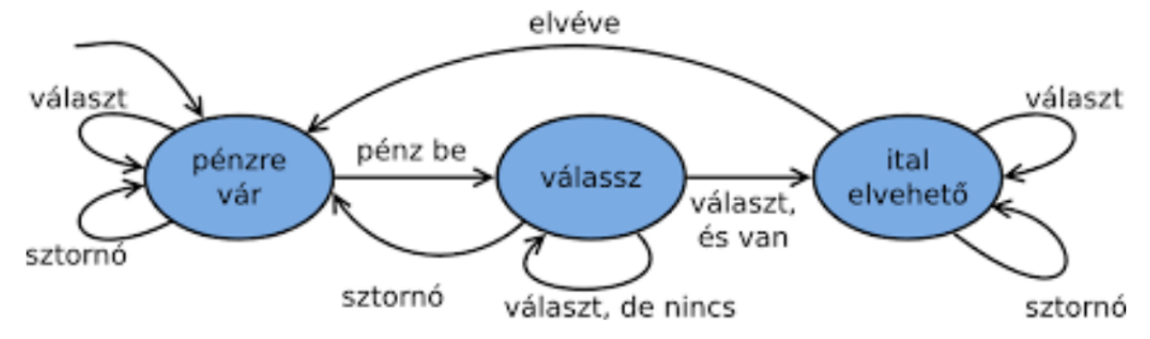
\includegraphics[width=0.8\textwidth]{res/imgs/info_29_state_machine.png}
    \end{center}
    \item \textbf{az állapotok:}
    \begin{itemize}
        \item pénzre vár (0)
        \item válassz (1)
        \item ital elvehető (2)
    \end{itemize}
    \item \textbf{események:}
    \begin{itemize}
        \item pénz be
        \item választ, és van
        \item választ és nincs
        \item elvéve
        \item sztornó
    \end{itemize}
    \item a megjelenítés miatt érdemes grafikus felületet programozni
    \item grafikus felület program felépítése (esemény vezérelt):
    \begin{enumerate}
        \item program indul (kezdeti inicializálás)
        \item program végtelen ciklusban várakozik
        \item az operációs rendszerben történik valami (esemény)
        \item A program erre az eseményre reagál valamely programrészlet (függvény, vagy metódus) végrehajtásával. Ha voltak a felületen bemenő adatok, azokat beolvassa, eredményeket számít, majd megjelenít a felületen.
        \item várakozik (2. lépés) vagy amíg a ,,lépj ki'' esemény meg nem érkezik
        \item kilép
    \end{enumerate}
    \item hozzunk létre egy állapotváltozót, mely csak az állapotokhoz tartozó általunk előre kiválasztott értékeket veheti fel, ha mást venne fel, lépjen ki a program
    \item az eseményeinket könnyen tudjuk gombokkal kezelni
    \item az állapotok megjeleníthetők label-lel, vagy pictureBox-szal
    \item írjunk egy függvényt:
    \begin{itemize}
        \item argumentumában legyen az aktuális állapot, valamint az esemény, ami éppen történt
        \item törzsében az utasítás legyen az, hogy ha az esemény az aktuális állapotot megváltoztatná, léptesse az állapotot a következő állapotra, valamint az állapothoz köthető tevékenységet hajtsa végre
    \end{itemize}
    \item a függvényt hívjuk meg minden alkalommal, amikor valamilyen esemény történik
\end{itemize}

\textbf{ARMA-modell:}
\begin{itemize}
    \item AutoRegresszív Mozgó Átlag
    \item általános alak:
    \begin{equation*}
        \sum_{i=0}^n a_{di} y[k-i] = \sum_{i=0}^r b_{di} u[k-i]
    \end{equation*}
    \item átrendezve a kimenet új értéke:
    \begin{equation*}
        y[k] = \sum_{i=0}^r b_{di} u[k-i] - \sum_{i=1}^n a_{di} y[k-i], \quad \text{ahol } a_{d0} = 1 \text{: az } y[k] \text{ együtthatója}
    \end{equation*}
    \item \textbf{AR} -- az $y[k]$ kimenő jel korábbi értékei hogyan hatnak vissza a kimenő jel aktuális értékeire
    \item \textbf{MA} -- az $u[k]$ bemenő jel korábbi értékei (mozgó átlaga) milyen hatással bírnak az aktuális kimenetre
\end{itemize}

\textbf{ARMA-modell programozás:}
\begin{itemize}
    \item $a$: $n$ méretű vektor (mivel $y[k]$ együtthatója 1), ismerjük
    \item $b$: egy $r+1$ méretű vektor, ismerjük
    \item hozzuk létre az $u$ bemeneti vektort, melynek ismerjük a bemeneteit
    \item tegyük fel, hogy a nulladik időpillanat előtt nem volt semmilyen bemenete a rendszernek
    \item innen kétféle módon tudunk számolni
    \begin{itemize}
        \item ha ki szeretnénk minden időpillanat kimenetét számolni, akkor for ciklusok segítségével mindig kiszámoljuk az adott elemet az eddigi adataink összegzésével, a kapott kimenetet pedig eltároljuk a vektorban
        \item ha csak egy adott időpillanat kimenetére vagyunk kíváncsiak, akkor írjunk egy függvényt, mely magát hívja meg -- így rekurzióval el tudunk jutni a kezdeti feltételig, ahonnan ki tudjuk számolni a keresett kimenetet
    \end{itemize}
\end{itemize}